\sloppy
Python Decision Making \par
\vspace{12pt}
\noindent 
Pengambilan keputusan adalah antisipasi kondisi yang terjadi saat pelaksanaan program dan menentukan tindakan yang dilakukan sesuai kondisi. \par
\vspace{12pt}
\noindent 
Struktur keputusan mengevaluasi banyak ekspresi yang menghasilkan TRUE atau FALSE sebagai hasil. \$  \$Anda perlu menentukan tindakan mana yang harus diambil dan pernyataan mana yang akan dijalankan jika hasilnya BENAR atau SALAH sebaliknya. \par
\vspace{12pt}
\noindent 
Berikut adalah bentuk umum dari struktur pengambilan keputusan yang khas atau khusus yang ditemukan di sebagian besar bahasa pemrograman
\ref{struktur}.
\begin{figure}[ht]
    \centerline{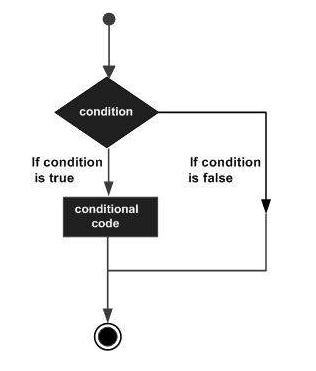
\includegraphics[width=0.25\textwidth]{figures/struktur.png}}
    \caption{struktur pada python}
    \label{struktur}
    \end{figure}\par
\vspace{12pt}
\noindent 
Decision making / Pemilihan keputusan pada python sangat penting untuk pemrograman komputer. Akan ada banyak situasi saat Anda diberi dua pilihan atau lebih dan Anda harus memilih opsi berdasarkan kondisi yang diberikan. Misalnya,
\begin{enumerate} \par
\item
Seorang murid dengan nilai lebih dari 90 disebut siswa pintar \par
\item
Seorang murid dengan nilai dibawah 90 dan diatas 30 disebut Siswa Standard \par
\item
Seorang murid dengan nilai dibawah 30 disebut siswa bodoh \par
\end{enumerate}\par
\vspace{12pt}
\noindent 
Bahasa pemrograman Python mengasumsikan nilai \$  \$non-nol \$  \$dan \$  \$non-nullsebagai TRUE, dan jika itu adalah \$  \$nol \$  \$atau \$  \$nol \$  \$, maka diasumsikan sebagai nilai FALSE. \par
\vspace{12pt}
\noindent 
Bahasa pemrograman Python menyediakan jenis pernyataan pengambilan keputusan berikut. \par
\vspace{12pt}
\noindent 
Mari kita membahas setiap keputusan secara singkat  \par
\vspace{12pt}
\noindent 
Setelah tutorial mengenai \$ 
{variable dan operator}
\$pada bahasa pemrograman python akan membahas mengenai percabangan/pengambilan keputusan. Percabangan atau pengambilan keputusan adalah pengkondisian yang terjadi ketika aplikasi berjalan, kemudian ada aksi-aksi tertentu atau kondisi tertentu sehingga aplikasi harus bereaksi terhadap hal itu. Atau dalam bahasa pemrograman umum dikenal dengan IF, THEN, ELSE sebagai contoh pengaplikasian dari pengambilan keputusan ini. \par
\vspace{12pt}
if statements
Sebuah if statement terdiri dari ekspresi boolean diikuti oleh satu atau lebih pernyataan.
\noindent 
Pada tulisan ini, saya menggunakan perangkat raspberry pi 2 dengan sistem operasi rasbian jessie. Sangat ringan dan tentunya python secara default ada di dalamnya. Kebetulan dalam tulisan ini masih menggunakan python versi 2, meskipun ada python versi 3 juga. \par
\vspace{12pt}
\noindent 
Python core tidak menyediakan  \$ \" \$switch \$ \" \$ atau  \$ " \$case \$ \" \$ seperti bahasa pemrograman lain. Tapi kita bisa menggunakan statemen if, elif yang bisa menggantikan  \$ \" \$switch \$ \" \$ atau  \$ \" \$case \$ \" \$. \par
\vspace{12pt}
\noindent 
Di bawah ini merupakan tipe-tipe percabangan yang disediakan oleh python. \par
\vspace{12pt}
\noindent 
IF : Mengandung expresi boolean dan diikuti oleh satu atau banyak statemen \par
\vspace{12pt}
\noindent 
IF ELSE : IF bisa diikuti oleh optional statemen yaitu ELSE, yang akan dieksekusi ketika ekspresi boolean bernilai FALSE \par
\vspace{12pt}
\noindent 
NESTED IF atau IF bersarang :~ Kita bisa menggunakan IF, ELSE IF di dalam IF, ELSE IF lainnya \par
\vspace{12pt}
\noindent 
Contoh dalam python untuk IF :  \par
\vspace{12pt}
\noindent 
varAngka1 = 123 \par
\vspace{12pt}
\noindent 
varAngka2 = 0 \par
\vspace{12pt}
\noindent 
if varAngka1: \par
\vspace{12pt}
\noindent 
 \$  \$ \$  \$ \$  \$ \$  \$ \$ \$ \$  \$ \$  \$ \$  \$ \$  \$ \$  \$ \$  \$ \$  \$ \$  \$ \$  \$ \$  \$ \$  \$print "Nilai : TRUE" \par
\vspace{12pt}
\noindent 
 \$  \$ \$  \$ \$  \$ \$  \$ \$  \$ \$  \$ \$  \$ \$  \$ \$  \$ \$  \$ \$  \$ \$  \$ \$  \$ \$  \$ \$  \$ \$  \$print varAngka1 \par
\vspace{12pt}
\noindent 
if varAngka2: \par
\vspace{12pt}
\noindent 
 \$  \$ \$  \$ \$  \$ \$  \$ \$ \$ \$  \$ \$  \$ \$  \$ \$  \$ \$  \$ \$  \$ \$  \$ \$  \$ \$  \$ \$  \$ \$  \$print "Nilai : TRUE" \par
\vspace{12pt}
\noindent 
 \$  \$ \$  \$ \$  \$ \$  \$ \$ \$ \$  \$ \$  \$ \$  \$ \$  \$ \$  \$ \$  \$ \$  \$ \$  \$ \$  \$ \$  \$ \$  \$print varAngka2{\fontsize{14pt}{14pt}\selectfont  \$  \$ \\} \par
\vspace{12pt}
\noindent 
Contoh untuk IF ELIF ELSE, di python sintak ini bisa ditulis dengan lebih singkat yaitu elif :  \par
\vspace{12pt}
\noindent 
varAngka = 123 \par
\noindent 
 $  $ \par
\noindent 
if varAngka==200: \par
\vspace{12pt}
\noindent 
 $  $  $  $  $  $  $  $  $  $  $  $  $  $print "Nilai : TRUE" \par
\vspace{12pt}
\noindent 
 $  $  $  $  $  $  $  $  $  $  $  $  $  $print varAngka \par
\vspace{12pt}
\noindent 
elif varAngka==123: \par
\vspace{12pt}
\noindent 
 $  $  $  $  $  $  $  $  $  $  $  $  $  $print "Nilai : TRUE" \par
\vspace{12pt}
\noindent 
 $  $  $  $  $  $  $  $  $  $  $  $  $  $print varAngka \par
\vspace{12pt}
\noindent 
else: \par
\vspace{12pt}
\noindent 
 $  $  $  $  $  $  $  $  $  $  $  $  $  $print "Nilai : FALSE" \par
\vspace{12pt}
\noindent 
 $  $  $  $  $  $  $  $  $  $  $  $  $  $print varAngka \par
\vspace{12pt}
\noindent 
Contoh untuk NESTED IF :  \par
\vspace{12pt}
\noindent 
varAngka = 89 \par
\noindent 
 $  $ \par
\noindent 
if varAngka<100: \par
\vspace{12pt}
\noindent 
 $  $  $  $  $  $  $  $  $  $  $  $print "Nilai : TRUE" \par
\vspace{12pt}
\noindent 
 $  $  $  $  $  $  $  $  $  $  $  $print varAngka \par
\vspace{12pt}
\noindent 
 $  $  $  $  $  $  $  $  $  $  $  $if varAngka > 80: \par
\vspace{12pt}
\noindent 
 $  $  $  $  $  $  $  $  $  $  $  $  $  $  $  $  $  $  $  $  $  $  $  $ print "Nilai : A" \par
\vspace{12pt}
\noindent 
 $  $  $  $  $  $  $  $  $  $  $  $elif varAngka > 60: \par
\vspace{12pt}
\noindent 
 $  $  $  $  $  $  $  $  $  $  $  $  $  $  $  $  $  $  $  $  $  $  $  $ print "Nilai : B" \par
\vspace{12pt}
\noindent 
 $  $  $  $  $  $  $  $  $  $  $  $elif varAngka > 40: \par
\vspace{12pt}
\noindent 
 $  $  $  $  $  $  $  $  $  $  $  $  $  $  $  $  $  $  $  $  $  $  $  $ print "Nilai : C" \par
\vspace{12pt}
\noindent 
 $  $  $  $  $  $  $  $  $  $  $  $elif varAngka > 20: \par
\vspace{12pt}
\noindent 
 $  $  $  $  $  $  $  $  $  $  $  $  $  $  $  $  $  $  $  $  $  $  $  $ print "Nilai : D" \par
\vspace{12pt}
\noindent 
 $  $  $  $  $  $  $  $  $  $  $  $else: \par
\vspace{12pt}
\noindent 
 $  $  $  $  $  $  $  $  $  $  $  $  $  $  $  $  $  $  $  $  $  $  $  $ print "Nilai : E" \par
\vspace{12pt}
\noindent 
else: \par
\vspace{12pt}
\noindent 
 $  $  $  $  $  $  $  $  $  $  $  $print "Nilai : FALSE" \par
\vspace{12pt}
\noindent 
 $  $  $  $  $  $  $  $  $  $  $  $print varAngka \par
\vspace{12pt}
\noindent 
Statemen IF juga bisa ditulis dalam 1 baris saja, misalnya seperti ini :  \par
\vspace{12pt}
\noindent 
if varAngka1: print "Nilai : TRUE" \par
\vspace{12pt}
\noindent 
Dari sintak percabangan sudah bisa kita lihat perbedaan antara python dengan bahasa pemrograman yang lain. Sintak ditulis dengan lebih ringkas. Percabangan atau pengkondisian ini adalah hal dasar dalam pemrograman, kita pasti akan menggunakannya. Pada artikel selanjutnya saya akan menulis mengenai perulangan atau looping dalam python. \par
\vspace{12pt}
\noindent 
Suite pernyataan tunggal \par
\vspace{12pt}
\noindent 
Jika rangkaian \$  \$klausa \$  \$jika \$  \$hanya terdiri dari satu baris, itu mungkin sama pada baris perintah sebagai pernyataan header. \par
\vspace{12pt}
\noindent 
Berikut adalah contoh \$  \$klausa \$  \$satu baris jika \$  \$- \par
\vspace{12pt}
\vspace{12pt}
\noindent 
var = 100 \par
\vspace{12pt}
\noindent 
if ( var~ == 100 ) : print "Value of expression is 100" \par
\vspace{12pt}
\noindent 
print "Good bye!" \par
\vspace{12pt}
\noindent 
Bila kode diatas dieksekusi, maka menghasilkan hasil sebagai berikut - \par
\vspace{12pt}
\noindent 
Value of expression is 100 \par
\vspace{12pt}
\noindent 
Good bye! \hspace*{1.31in}  \par
\noindent 
\vspace{12pt}
\noindent 
Pengambilan keputusan (kondisi if) digunakan untuk mengantisipasi kondisi yang terjadi saat jalanya program dan menentukan tindakan apa yang akan diambil sesuai dengan kondisi. \par
\noindent 
\vspace{12pt}
\noindent 
Pada python ada beberapa statement atau kondisi diantaranya adalah \$  \$if, \$  \$else \$  \$dan \$  \$elif \$  \$Kondisi \$  \$if \$  \$digunakan untuk mengeksekusi kode jika kondisi bernilai benar. \par
\noindent 
\vspace{12pt}
\noindent 
Jika kondisi bernilai salah maka statement atau kondisi if tidak akan di-eksekusi. \par
\noindent 
\vspace{\baselineskip}
Dibawah ini adalah contoh penggunaan kondisi if pada Python \par
\noindent 
\vspace{\baselineskip}
Dari contoh diatas, jika program dijalankan maka akan mencetak string \"Selamat Anda Lulus Ujian\" sebanyak 1 kali yaitu pada if pertama. Di if kedua statement bernilai salah, jadi perintah \$  \$print(\"Selamat Anda Lulus\") \$  \$tidak akan dieksekusi. \par
\noindent 
\vspace{\baselineskip}
Selanjutnya Anda bisa mempelajari kondisi if else \par
\vspace{12pt}
\noindent 
Pengambilan keputusan (kondisi if else) tidak hanya digunakan untuk menentukan tindakan apa yang akan diambil sesuai dengan kondisi, tetapi juga digunakan untuk menentukan tindakan apa yang akan diambil atau dijalankan jika kondisi tidak sesuai.\vspace{\baselineskip}
\vspace{\baselineskip}
 \par
\noindent 
Pada python ada beberapa statement atau kondisi diantaranya adalah \$  \$if, \$  \$else \$  \$dan \$  \$elif \$  \$Kondisi \$  \$if \$  \$digunakan untuk mengeksekusi kode jika kondisi bernilai benar.\vspace{\baselineskip}
\vspace{\baselineskip}
 \par
\noindent 
Kondisi if else adalah kondisi dimana jika pernyataan benar (true) maka kode dalam if akan dieksekusi, tetapi jika bernilai salah (false) maka akan mengeksekusi kode di dalam else.\vspace{\baselineskip}
\vspace{\baselineskip}
 \par
\noindent 
Dibawah ini adalah contoh penggunaan kondisi if else pada Python \par
\vspace{12pt}
\noindent 
Kondisi if else adalah jika kondisi bernilai TRUE maka akan dieksekusi pada if, tetapi jika bernilai FALSE maka akan dieksekusi kode pada else \par
\noindent 
\vspace{\baselineskip}
nilai = 3\vspace{\baselineskip}
 \par
\noindent 
Jika pernyataan pada if bernilai TRUE maka if akan dieksekusi, tetapi jika FALSE kode pada else yang akan dieksekusi.\vspace{\baselineskip}
 \par
\noindent 
if(nilai > 7):\vspace{\baselineskip}
 \$  \$  \$  \$ \par
\noindent 
 print(\"Selamat Anda Lulus\")\vspace{\baselineskip}
 \par
\noindent 
else:\vspace{\baselineskip}
 \par
\noindent 
 \$  \$  \$  \$ print(\"Maaf Anda Tidak Lulus\") \par
\noindent 
\vspace{\baselineskip}
\vspace{\baselineskip}
Pada contoh diatas, jika program dijalankan maka akan mencetak string \"Maaf Anda Tidak Lulus\" karena pernyataan pada if bernilai FALSE \par
\noindent 
\vspace{\baselineskip}
Selanjutnya kita akan mempelajari per-kondisi an pada python yang terakhir yaitu \"Elif\" \$  \$ \par
\vspace{12pt}
\noindent 
Pengambilan keputusan (kondisi if elif) merupakan lanjutan atau percabangan logika dari \"kondisi if\". Dengan elif kita bisa membuat kode program yang akan menyeleksi beberapa kemungkinan yang bisa terjadi. Hampir sama dengan kondisi \"else\", bedanya kondisi \"elif\" bisa banyak dan tidak hanya satu. \$  \$\vspace{\baselineskip}
\vspace{\baselineskip}
Dibawah ini adalah contoh penggunaan kondisi elif pada Python \par
\vspace{12pt}
\noindent 
Contoh penggunaan kondisi elif \par
\vspace{12pt}
\noindent 
hari \$  \_  \$ini = \"Minggu\" \par
\noindent 
\vspace{\baselineskip}
\vspace{\baselineskip}
if(hari \$  \_  \$ini == \"Senin\"): \par
\noindent 
\vspace{\baselineskip}
 \$  \$  \$  \$ print(\"Saya akan kuliah\") \par
\noindent 
\vspace{\baselineskip}
elif(hari \$  \_  \$ini == \"Selasa\"): \par
\noindent 
\vspace{\baselineskip}
 \$  \$  \$  \$ print(\"Saya akan kuliah\") \par
\noindent 
\vspace{\baselineskip}
elif(hari \$  \_  \$ini == \"Rabu\"): \par
\noindent 
\vspace{\baselineskip}
 \$  \$  \$  \$ print(\"Saya akan kuliah\") \par
\noindent 
\vspace{\baselineskip}
elif(hari $  \_  $ini == "Kamis"): \par
\noindent 
\vspace{\baselineskip}
 $  $  $  $ print("Saya akan kuliah") \par
\noindent 
\vspace{\baselineskip}
elif(hari $  \_  $ini == "Jumat"): \par
\noindent 
\vspace{\baselineskip}
 $  $  $  $ print("Saya akan kuliah") \par
\noindent 
\vspace{\baselineskip}
elif(hari $  \_  $ini == "Sabtu"): \par
\noindent 
\vspace{\baselineskip}
 $  $  $  $ print("Saya akan kuliah") \par
\noindent 
\vspace{\baselineskip}
elif(hari $  \_  $ini == "Minggu"): \par
\noindent 
\vspace{\baselineskip}
 $  $  $  $ print("Saya akan libur") \par
\noindent 
\vspace{\baselineskip}
\vspace{\baselineskip}
Pada contoh diatas, jika program dijalankan maka akan mencetak \$  
\$\"Saya akan libur\". \par
\noindent 
 \$  \$ Pernyataan digunakan untuk pengambilan keputusan dalam python berupa if, pernyataan tersebut memiliki format lengkap sebagai berikut : \par
\vspace{12pt}
\noindent 
~~~ if kondisi \$  \_  \$1: \par
\vspace{12pt}
\noindent 
~~~~~~ pernyataan \$  \_  \$pernyataan \$  \_  \$1 \par
\vspace{12pt}
\noindent 
~~~ elif kondisi \$  \_  \$2: \par
\vspace{12pt}
\noindent 
~~~~~~ pernyataan \$  \_  \$pernyataan \$  \_  \$2 \par
\vspace{12pt}
\noindent 
~~~ elif kondisi \$  \_  \$3: \par
\vspace{12pt}
\noindent 
~~~~~~ pernyataan \$  \_  \$pernyataan \$  \_  \$3 \par
\vspace{12pt}
\noindent 
~~~ else kondisi \$  \_  \$n: \par
\vspace{12pt}
\noindent 
~~~~~~ pernyataan \$  \_  \$pernyataan-n \par
\vspace{12pt}
\noindent 
~~~~~~  \par
\noindent 
~~~ if kondisi \$  \_  \$1,elif kondisi \$  \_  \$2,elif kondisi \$  \_  \$3,else kondisi \$  \_  \$n \par
\vspace{12pt}
\noindent 
~~~~berupa~suatu ekspresi yang menghasilkan nilai logika (benar atau salah)    \par
\noindent 
~~~  \par
\noindent 
Contoh Code dijalankan pada modus interaktif \par
\vspace{12pt}
\noindent 
  x = 5 \par
\vspace{12pt}
\noindent 
~ y = 100 \par
\vspace{12pt}
\noindent 
~~~ terbesar = x \par
\vspace{12pt}
\noindent 
~~ if terbesar < y: \par
\vspace{12pt}
\noindent 
terbesar = y \par
\vspace{12pt}
~~~ terbesar = 100  \par
\vspace{12pt}
\noindent 
~~~  \par
\vspace{12pt}
\noindent 
 \$ \$Python tidak menggunakan \$ \{ \$ \$ \} \$ untuk menyertakan blok kode untuk penggunaan if or loop or fungsi dll. Sebaliknya, python menggunakan titik dua (:) dan indentasi atau spasi untuk pernyataan \$ \$kelompok. Tes \$ \$boolean untuk if tidak perlu dalam tanda kurung (perbedaan besar dari C++ atau Java), dan dapat memiliki *elif* dan *else*. \par
\noindent 
\vspace{\baselineskip}
 \$  \$ \$  \$ \$  \$ \$  \$Nilai apapun dapat digunakan sebagai if-test. pada  \$ \" \$nol \$ \" \$ nilai-nilai semua dihitung sebagai false:Tidak ada,0,string kosong,list kosong, dictionary kosong. Ada juga tipe Boolean dengan dua nilai: True dan False (jika dikonversi ke int, ini adalah 1 dan 0). Python memiliki operasi perbandingan yang biasa: ==, =, <, <=,>,> =. Tidak seperti Java dan C.Operator boolean bisa juga di eja seperti * and *, * or *, * not * (Python tidak menggunakan gaya C  \$  \&  \$  \$  \&  \$  \$  \vert  \$  \$  \vert  \$!). \par
\vspace{12pt}
\noindent 
~~~~matakuliah = 'matematika'   matematika,fisika \par
\noindent 
~~  \par
\noindent 
 nilai = 70 100,80,50 \par
\vspace{12pt}
\noindent 
~~~ if nilai >=100 or nilai>=80 : \par
\vspace{12pt}
\noindent 
~~~~~~ if matakuliah == 'matematika': \par
\vspace{12pt}
\noindent 
~~~~~~~~~ print 'anda mendapat nilai A dalam mata kuliah matematika' \par
\vspace{12pt}
\noindent 
~~~ elif matakuliah == 'fisika': \par
\vspace{12pt}
\noindent 
~~~~~~ print 'anda mendapat nilai A dalam mata kuliah Fisika' \par
\vspace{12pt}
\noindent 
~~~ elif nilai >=70 and matakuliah=='matematika': \par
\vspace{12pt}
\vspace{12pt}
\noindent 
~~~~~~ print 'anda mendapat nilai B dalam mata kuliah matematika' \par
\vspace{12pt}
\noindent 
~~~ elif nilai >=70 and matakuliah=='fisika': \par
\vspace{12pt}
\noindent 
~~~~~~ print 'anda mendapat nilai B dalam mata kuliah fisika' \par
\vspace{12pt}
\noindent 
~~~ else: \par
\vspace{12pt}
\noindent 
~~~~~~ print 'nilai dan~matakuliah~tidak~ada'~~~     \par
\vspace{12pt}
\noindent 
Seperti halnya bahasa pemrograman yang lain, tentu python juga mempunyai perintah untuk pengambilan suatu keputusan terhadap kondisi tertentu, yang disebut percabangan. Percabangan pada bahasa pemrograman python menggunakan perintah if, ya sama dengan bahasa pemrograman yang lain. Bagaimana cara menggunakan perintah if ini dalam bahasa pemrograman python? \par
\noindent 
\vspace{\baselineskip}
Cara penulisan dari perintah if secara garis besar adalah seperti berikut: \par
\noindent 
\vspace{\baselineskip}
\vspace{\baselineskip}
if <kondisi 1>: \par
\noindent 
\vspace{\baselineskip}
 \$  \$<perintah yang dijalankan 1> \par
\noindent 
\vspace{\baselineskip}
elif <kondisi 2>: \par
\noindent 
\vspace{\baselineskip}
<perintah yang dijalankan 2> \par
\noindent 
\vspace{\baselineskip}
else:\vspace{\baselineskip}
 \$  \$<perintah yang dijalankan 3> \par
\noindent 
\vspace{\baselineskip}
\vspace{\baselineskip}
Perintah-perintah yang dipergunakan antara lain \par
\noindent 
\vspace{\baselineskip}
If dan If bersarang \par
\noindent 
\vspace{\baselineskip}
Elif (singkatan dari: else if) dan \par
\noindent 
\vspace{\baselineskip}
else.\vspace{\baselineskip}
 \par
\noindent 
\vspace{\baselineskip}
IF Bersarang \par
\noindent 
\vspace{\baselineskip}
Adapun tanda titik dua diletakan setelah kondisi, sedangkan untuk perintah yang dijalankan jika kondisi if terpenuhi diberi tab atau 4 spasi pada depannya untuk menandakan bahwa perintah tersebut berada didalam if, contoh dalam source code. Misal kita ingin menentukan angka genap atau ganjil: \par
\noindent 
\vspace{\baselineskip}
angka = 7 \par
\noindent 
\vspace{\baselineskip}
if angka  $  \%  $ 2 == 0: \par
\noindent 
\vspace{\baselineskip}
 $  $  $  $ print 'genap' \par
\noindent 
\vspace{\baselineskip}
else:\vspace{\baselineskip}
 $  $print 'ganjil' \par
\noindent 
\vspace{\baselineskip}
 Dari perintah diatas akan menghasilkan nilai yang diprint adalah 'ganjil'. Tanda  $  \%  $ (persen) disini merupakan operator untuk modulus, yaitu sisa bagi. Adapun jalannya dari program diatas adalah, jika angka dalam hal ini nilainya 7 jika di modulus dengan 2, menyisahkan nilai nol maka data yang diprint adalah genap, jika tidak menyisahkan nilai nol maka data yang diprint adalah ganjil. \par
\noindent 
\vspace{\baselineskip}
Bagaimana halnya dengan kondisi yang lebih dari satu. Misal kita ingin menentukan game yang kita sukai: \par
\noindent 
\vspace{\baselineskip}
pilihan = 2 \par
\noindent 
\vspace{\baselineskip}
if pilihan == 1: \par
\noindent 
\vspace{\baselineskip}
 $  $  $  $ print 'DOTA2' \par
\noindent 
\vspace{\baselineskip}
else:\vspace{\baselineskip}
 $  $  $  $ if pilihan == 2: \par
\noindent 
\vspace{\baselineskip}
 $  $  $  $  $  $  $  $ print 'GTA V Online' \par
\noindent 
\vspace{\baselineskip}
 $  $  $  $ else: \par
\noindent 
\vspace{\baselineskip}
 $  $  $  $  $  $  $  $ print 'Semua Game' \par
\noindent 
\vspace{\baselineskip}
Perintah diatas merupakan if bersarang yaitu terdapat if didalam if, dapat juga dituliskan dengan perintah dibawah ini dengan menggunakan elif: \par
\noindent 
\vspace{\baselineskip}
\vspace{\baselineskip}
Elif \par
\noindent 
\vspace{\baselineskip}
Merupakan suatu pemilihan kondisi dimana dalam kondisi tersebut, terdapat lagi kondisi lain\vspace{\baselineskip}
Contoh kodingnya : \par
\noindent 
\vspace{\baselineskip}
Program Kategori Berat hewan qurban \par
\noindent 
\vspace{\baselineskip}
pilihan = 300 \par
\noindent 
\vspace{\baselineskip}
if pilihan > 300: \par
\noindent 
\vspace{\baselineskip}
 $  $  $  $ print 'Sapi boleh diqurban' \par
\noindent 
\vspace{\baselineskip}
elif pilihan <  $  $300 : \par
\noindent 
\vspace{\baselineskip}
 $  $  $  $ print 'Sapi belum boleh diqurban' \par
\noindent 
\vspace{\baselineskip}
else: \par
\noindent 
\vspace{\baselineskip}
 $  $  $  $ print ‘Rawat dulu sapinya yang benar' \par
\noindent 
\vspace{\baselineskip}
Mana yang terbaik dari kedua cara penulisan kondisi if yang lebih dari satu diatas itu tentunya sesuai dengan kebutuhan kita masing-masing dalam membuat suatu aplikasi. Dalam if pun kita bisa membuat dua atau lebih persyaratan dalam kondisi if \par
\noindent 
\vspace{\baselineskip}
\vspace{\baselineskip}
Else \par
\noindent 
\vspace{\baselineskip}
contohnya:\vspace{\baselineskip}
angka = 2 \par
\noindent 
\vspace{\baselineskip}
if angka <= 10 and angka >= 1 : \par
\noindent 
\vspace{\baselineskip}
 $  $  $  $ print 'angka diantara 1 dan 10' \par
\noindent 
\vspace{\baselineskip}
else: \par
\noindent 
\vspace{\baselineskip}
 $  $  $  $ print 'angka diluar jangkauan' \par
\vspace{12pt}
\noindent 
Percabangan Pada Bahasa Pemrograman Python. \par
\vspace{12pt}
\noindent 
Seperti halnya bahasa pemrograman yang lain, tentu python juga mempunyai perintah untuk pengambilan suatu keputusan terhadap kondisi tertentu, yang disebut percabangan. Percabangan pada bahasa pemrograman python menggunakan perintah $  $if, ya sama dengan bahasa pemrograman yang lain. Bagaimana cara menggunakan perintah $  $if $  $ini dalam bahasa pemrograman python? Yuk mari kita sama-sama melihat cara penggunaan perintah $  $if $  $ini. \par
\vspace{12pt}
\noindent 
Cara penulisan dari perintah if secara garis besar adalah seperti berikut: \par
\noindent 
if <kondisi 1>: \par
\vspace{12pt}
\noindent 
~~~ <perintah yang dijalankan 1> \par
\vspace{12pt}
\noindent 
elif <kondisi 2>: \par
\vspace{12pt}
\noindent 
~~~ <perintah yang dijalankan 2> \par
\vspace{12pt}
\noindent 
else: \par
\vspace{12pt}
\noindent 
~~~ <perintah yang dijalankan 3> \par
\vspace{12pt}
\noindent 
Perintah-perintah yang dipergunakan antara lain $  $if, $  $elif $  $(singkatan dari: $  $else if) dan $  $else. Adapun tanda titik dua diletakan setelah kondisi, sedangkan untuk perintah yang dijalankan jika kondisi if terpenuhi diberi $  $tab $  $atau $  $4 spasi $  $pada depannya untuk menandakan bahwa perintah tersebut berada didalam if, contoh dalam source code. Misal kita ingin menentukan angka genap atau ganjil: \par
\vspace{12pt}
\noindent 
angka = 7 \par
\vspace{12pt}
\noindent 
if angka  $  \%  $ 2 == 0: \par
\vspace{12pt}
\noindent 
~~~ print 'genap' \par
\vspace{12pt}
\noindent 
else: \par
\vspace{12pt}
\noindent 
~~~ print 'ganjil' \par
\vspace{12pt}
\noindent 
Dari perintah diatas akan menghasilkan nilai yang diprint adalah 'ganjil'. Tanda $  $ $  \%  $ $  $(persen) disini merupakan operator untuk modulus, yaitu sisa bagi. Adapun jalannya dari program diatas adalah, jika angka dalam hal ini nilainya 7 jika di modulus dengan 2, menyisahkan nilai nol maka data yang diprint adalah genap, jika tidak menyisahkan nilai nol maka data yang diprint adalah ganjil. \par
\vspace{12pt}
\noindent 
Bagaimana halnya dengan kondisi yang lebih dari satu. Misal kita ingin menentukan buah yang kita sukai: \par
\vspace{12pt}
\noindent 
pilihan = 2 \par
\vspace{12pt}
\noindent 
if pilihan == 1: \par
\vspace{12pt}
\noindent 
~~~ print 'buah durian' \par
\vspace{12pt}
\noindent 
else: \par
\vspace{12pt}
\noindent 
~~~ if pilihan == 2: \par
\vspace{12pt}
\noindent 
~~~~~~~ print 'buah mangga' \par
\vspace{12pt}
\noindent 
~~~ else: \par
\vspace{12pt}
\noindent 
~~~~~~~ print 'semua buah' \par
\vspace{12pt}
\noindent 
Perintah diatas merupakan if bersarang yaitu terdapat if didalam if, dapat juga dituliskan dengan perintah dibawah ini dengan menggunakan $  $elif: \par
\vspace{12pt}
\noindent 
pilihan = 2 \par
\vspace{12pt}
\noindent 
if pilihan == 1: \par
\vspace{12pt}
\noindent 
~~~ print 'buah durian' \par
\vspace{12pt}
\noindent 
elif pilihan == 2: \par
\vspace{12pt}
\noindent 
~~~ print 'buah mangga' \par
\vspace{12pt}
\noindent 
else: \par
\vspace{12pt}
\noindent 
~~~ print 'semua buah' \par
\vspace{12pt}
\noindent 
Mana yang terbaik dari kedua cara penulisan kondisi if yang lebih dari satu diatas itu tentunya sesuai dengan kebutuhan kita masing-masing dalam membuat suatu aplikasi, seperti kata orang, banyak jalan menuju roma begitu juga dengan pemrograman, banyak jalan untuk menuliskan suatu perintah untuk menghasilkan hasil tertentu... :) \par
\vspace{12pt}
\noindent 
Dalam if pun kita bisa membuat dua atau lebih persyaratan dalam kondisi $  $if $  $contohnya: \par
\vspace{12pt}
\noindent 
angka = 2 \par
\vspace{12pt}
\noindent 
if angka <= 10 and angka >= 1 : \par
\vspace{12pt}
\noindent 
~~~ print 'angka diantara 1 dan 10' \par
\vspace{12pt}
\noindent 
else: \par
\vspace{12pt}
\noindent 
~~~ print 'angka diluar jangkauan' \par
\vspace{12pt}
\vspace{12pt}

